% =============================================================================
% File:  sample_slides.tex --  Example of the use of the Falkor Beamer theme
% Author(s): Sebastien Varrette <Sebastien.Varrette@uni.lu>
% Time-stamp: <Mar 2014-04-29 16:06 svarrette>
% 
% Copyright (c) 2012 Sebastien Varrette <Sebastien.Varrette@uni.lu>
% .             http://varrette.gforge.uni.lu
% 
% For more information:
% - LaTeX: http://www.latex-project.org/
% - Beamer: https://bitbucket.org/rivanvx/beamer/
% - LaTeX symbol list:
% http://www.ctan.org/tex-archive/info/symbols/comprehensive/symbols-a4.pdf
% 
% Latest version of these files can be found on Github:
% 

% =============================================================================
\documentclass{beamer}
% \documentclass[draft]{beamer}
\usepackage{_style}
\usepackage{__config}

% The key part to use my theme
\usetheme{Falkor}

% Not integrated in my theme as not everybody wants that
\AtBeginSection[]
{
  \frame{
    \frametitle{Summary}
    {\scriptsize\tableofcontents[currentsection]}
  }
}

%%%%%%%%%%%%%%%%%%%%%%%%%%%% Header %%%%%%%%%%%%%%%%%%%%%%%%%%%%%%
\title{\EventName}
\subtitle{\TPindex: \TPtitle}

\author{\authors}
\institute[UL]{
  University of Luxembourg, Luxembourg
}

% Mandatory to define a logo - otherwise compilation will fail in an unobvious
% manner.
\pgfdeclareimage[height=0.8cm]{logo}{images/logo_UL.pdf}
\logo{\pgfuseimage{logo}}
\date{}

%%%%%%%%%%%%%%%%%%%%%%%%%%%%%% Body %%%%%%%%%%%%%%%%%%%%%%%%%%%%%%%
\begin{document}

\begin{frame}
    \vspace{2.5em}
    \titlepage
\end{frame}

% .......
\frame{
  \begin{center}
      \textbf{Latest versions available on
        \href{https://github.com/ULHPC/}{Github}}:
      \vfill
      \begin{description}
        \item[UL HPC tutorials:] \hfill
          \myurl{https://github.com/ULHPC/tutorials}
        \item[UL HPC School:] \hfill
          \myurl{http://hpc.uni.lu/hpc-school/}
        \item[\TPindex tutorial sources:] \hfill
          \myurl{\TPghurl}
      \end{description}
  \end{center}
}

% ......
\frame{
  \frametitle{Summary}
  {\scriptsize
    \tableofcontents
  }
}

% ===============================================
\section{Pre-requisites}

% .......
\begin{frame}[fragile]
\frametitle{Tutorial files}
  Sample MATLAB scripts used in the tutorial\\
  \begin{itemize}
   \item download only the scripts: \\
  \begin{cmdline}
    \cmdlinefrontend{mkdir \$HOME/matlab-tutorial} \\
    \cmdlinefrontend{cd \$HOME/matlab-tutorial} \\
    \cmdlinefrontend{wget \myurl{https://raw.github.com/ULHPC/tutorials/devel/advanced/MATLAB/example1.m}} \\
    \cmdlinefrontend{wget \myurl{https://raw.github.com/ULHPC/tutorials/devel/advanced/MATLAB/example2.m}} \\
    \cmdlinefrontend{wget \myurl{https://raw.github.com/ULHPC/tutorials/devel/advanced/MATLAB/yahoo\_finance\_data.m}} \\
  \end{cmdline}
  \item \textit{or} download the full repository and link to the MATLAB tutorial: \\
  \begin{cmdline}
    \cmdlinefrontend{git clone \myurl{https://github.com/ULHPC/tutorials.git}} \\
    \cmdlinefrontend{ln -s tutorials/advanced/MATLAB/ \$HOME/matlab-tutorial} \\
  \end{cmdline}  
  \end{itemize}

\end{frame}

\begin{frame}[fragile]
\frametitle{X Window System}
  In order to see locally the MATLAB graphical interface, \\
  a package providing the X Window System is required:
  \begin{itemize}
    \item on OS X: \textbf{XQuartz} \hfill\myurl{http://xquartz.macosforge.org/landing/}
    \item on Windows: \textbf{XMing} \hfill\myurl{http://sourceforge.net/projects/xming/}
  \end{itemize}
  \hfill \\ \hfill \\ %\hfill \\
  
  Now you will be able to connect with X11 forwarding enabled:
  \begin{itemize}
    \item on Linux \& OS X: \\
    \begin{cmdline}
       \cmdlineentry{ssh access-gaia.uni.lu} \textbf{-X}
    \end{cmdline}
    \item on Windows, with Putty \\
     Connection $\rightarrow$ SSH $\rightarrow$ X11 $\rightarrow$ \textbf{Enable X11 forwarding}
  \end{itemize}  
\end{frame}




% ===============================================
\section{Objectives}

% ............
\frame{

  \frametitle{Objectives of this PS}

  \begin{itemize}
    \item Better understand the usage of MATLAB on the \ULHPC
  \end{itemize}
  \begin{alertblock}{}
      \begin{itemize}
        \item running in interactive mode
          \begin{itemize}
              \itemhook with either the full graphical or the text-mode interface
          \end{itemize}
        \item running in passive mode
          \begin{itemize}
              \itemhook several ways of submitting MATLAB jobs
          \end{itemize}
	\item using script (.m) files
	\item plotting data, saving the plots to file
	\item taking advantage of some parallelization capabilities
          \begin{itemize}
              \itemhook use of \textbf{parfor}
              \itemhook use of GPU-enabled functions
          \end{itemize}
      \end{itemize}
  \end{alertblock}

}

\section{Example 1}

% .......
\frame{
  \frametitle{Scripts and plots}
  \textbf{example1.m}: non-interactive script that shows:
\begin{itemize}
 \item the use of a stopwatch timer
 \item how to use an external function (financial data retrieval)
 \item how to use different plotting methods
 \item how to export the plots in different graphic formats
\end{itemize} 
 \includegraphics[width=0.45\linewidth,keepaspectratio]{plots/example1-2dplot.eps}
 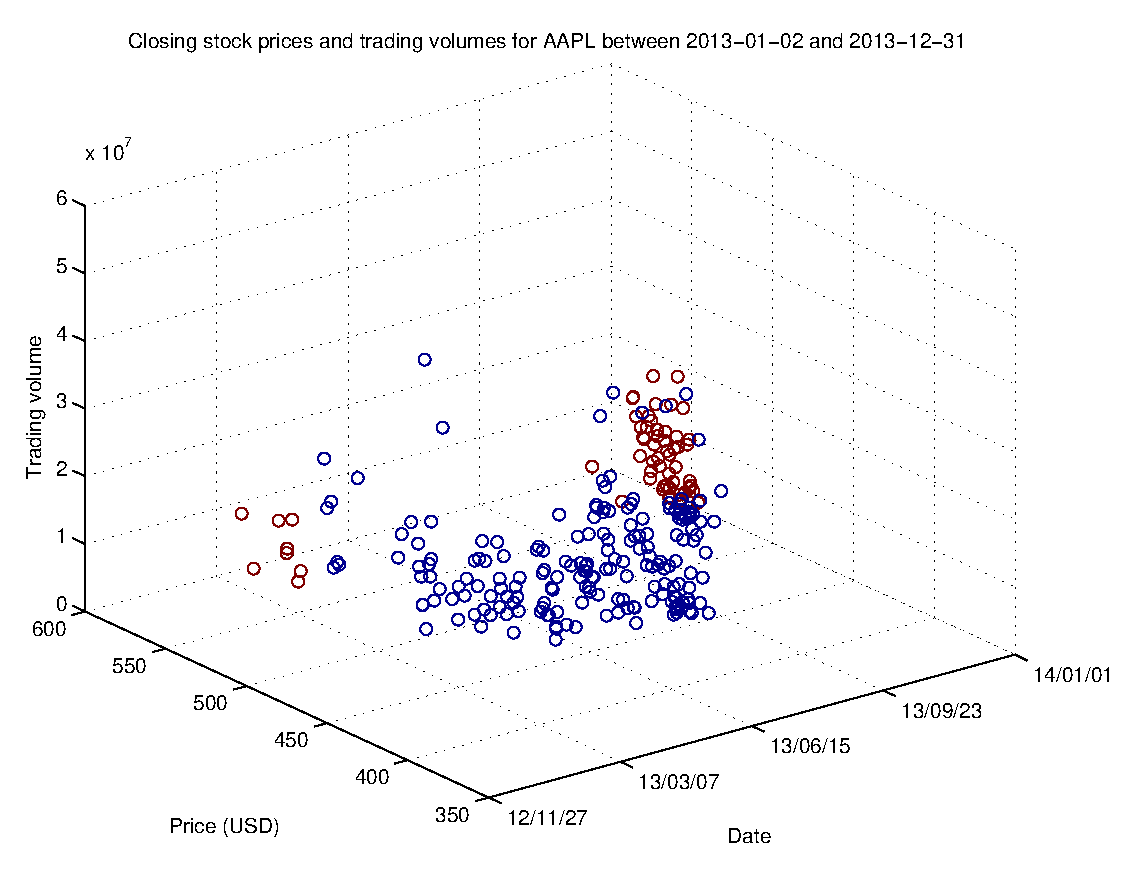
\includegraphics[width=0.45\linewidth,keepaspectratio]{plots/example1-scatter.eps}  
}

\section{Example 2}

% .......
\frame{
  \frametitle{Parallelization}
  \textbf{example2.m}: non-interactive script that shows:
  \begin{itemize}
   \item the serial execution of time consuming operations
   \item the parallel execution and relative speedup vs serial execution
   \item setting the \# of parallel threads through environment variables
   \item GPU-based parallel execution
  \end{itemize}
  \centering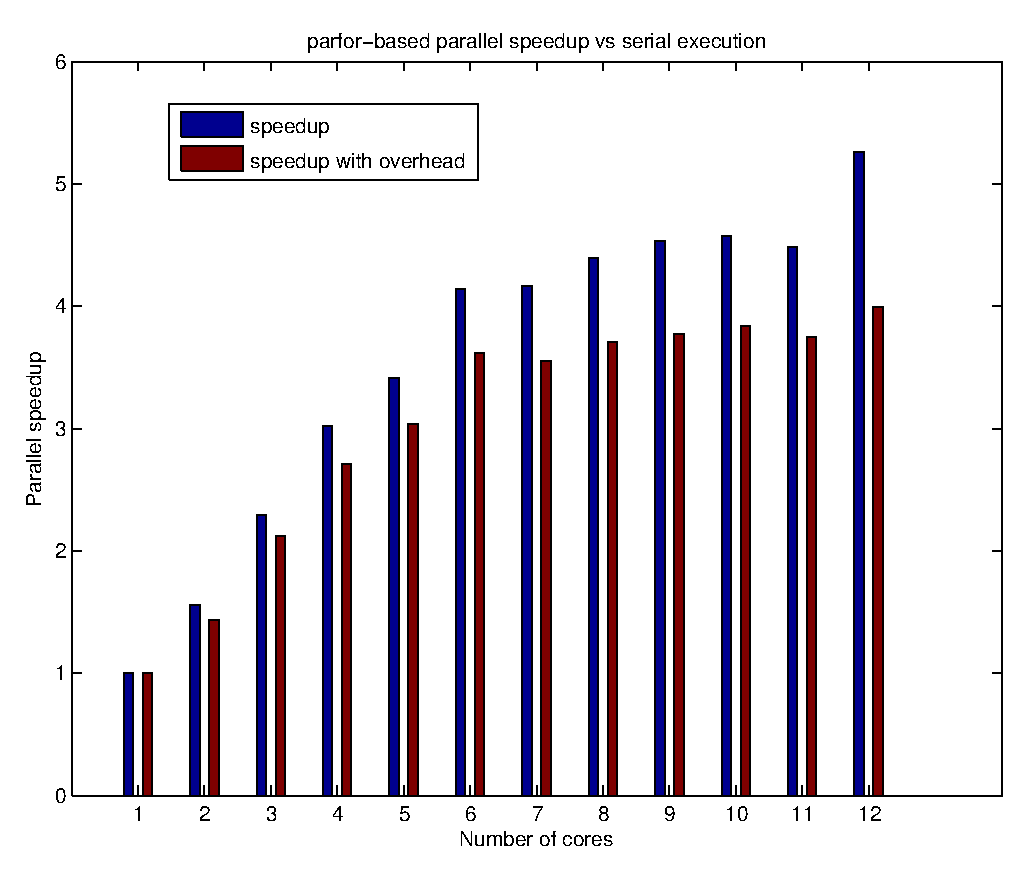
\includegraphics[width=0.45\linewidth,keepaspectratio]{plots/parfor-speedup.eps}
}


\section{Practical session}

% .......
\frame{
  \frametitle{Exercises}
    \begin{itemize}
      \item Read and understand the MATLAB tutorial \myurl{\TPghurl} \\
      $ \hookrightarrow $ \scriptsize{all provided scripts are fully commented}
      \item Run all the examples \\
      $ \hookrightarrow $ launching interactive/passive mode MATLAB \\
      $ \hookrightarrow $ plotting script \\
      $ \hookrightarrow $ parallel execution script \\
      \item Plot the speedup graph shown at \href{https://github.com/ULHPC/tutorials/tree/devel/advanced/MATLAB\#useful-references}{tutorial's end}
    \end{itemize}

}
\frame {
  \frametitle{Useful links}
  \begin{itemize}
   \item Parallel Computing Toolbox \hfill\myurl{http://www.mathworks.nl/help/distcomp/index.html}
   \item Parallel for-Loops (parfor) \hfill\myurl{http://www.mathworks.nl/help/distcomp/getting-started-with-parfor.html}
   \item GPU Computing \hfill\myurl{http://www.mathworks.nl/discovery/matlab-gpu.html}
  \end{itemize}
}  
\section{Conclusion}

% ............
\begin{frame}
  \frametitle{Conclusion}
  
  \begin{itemize}
    \item MATLAB execution modes on the \ULHPC
    \item Plotting and parallel execution
  \end{itemize}

    \begin{block}{Perspectives}
        \begin{itemize}
          \item Personalize the UL HPC launchers with the MATLAB commands
          \item Parallelize your own tasks using parfor/GPU-enabled instructions
        \end{itemize}
    \end{block}

\end{frame}

\section*{Thank you for your attention...}
\frame{
  \frametitle{Questions?}
  \begin{center}
      
\includegraphics[scale=0.2]{question.jpg}
  \end{center}

  {\tiny
    \tableofcontents

  }
}

\newcounter{finalframe}
\setcounter{finalframe}{\value{framenumber}}

% \appendix

% \frame{
%   \frametitle{Appendix}
% 
%   \begin{acronym}\setlength\itemsep{-0.3em}
%       \acro{DFT}{Discrete Fourier Transform}
%       \acro{EA}{Evolutionary Algorithm}
%       \acro{PRNG}{[Pseudo]-Random Number Generator}
%       \acro{UL}{University of Luxembourg}
%   \end{acronym}
% 
% }

\setcounter{framenumber}{\value{finalframe}}

\end{document}

% ~~~~~~~~~~~~~~~~~~~~~~~~~~~~~~~~~~~~~~~~~~~~~~~~~~~~~~~~~~~~~~~~
% eof
% 
% Local Variables:
% mode: latex
% mode: flyspell
% mode: auto-fill
% fill-column: 80
% End:
